% ----------------------------------------------------------
% Fundamentação Teórica
% ----------------------------------------------------------
\chapter{Fundamentação Teórica} \label{cha:fundamentacao}

Título de um capítulo é chamado seção primária. Deve ser em negrito e letras maiúsculas e sempre no topo de uma nova página. 

Texto da Associação Brasileira de Normas Técnicas (ABNT) texto texto texto texto texto texto texto texto texto texto texto texto texto texto texto texto texto texto texto texto texto texto texto texto texto texto texto texto texto texto texto texto texto 
texto.


\section{Título da Seção SECUNDÁRIA}
As políticas públicas são princípios norteadores, diretrizes para ações do 
poder público para com a sociedade. Faz-se necessário para tanto o seu 
entendimento, para Teixeira (2002, p. 2, aspas do autor),

\begin{citacao}
As citações diretas, no texto, com mais de três linhas, devem ser
destacadas com recuo de 4 cm da margem esquerda, com letra menor que a do texto
utilizado e sem as aspas. No caso de documentos datilografados, deve-se
observar apenas o recuo \cite[5.3]{NBR10520:2002}.
\end{citacao}

Neste entendimento percebe-se a importância da existência das políticas 
públicas, pois norteiam as ações desenvolvidas pelo Estado para atender as 
demandas da sociedade a qual serve. Possibilitando atingir pontos a serem cobertos 
que por quaisquer motivos, seja de ordem política, econômica ou social não tenha 
sido contemplados e que foram delineados em um certo contexto histórico-social. O 
Estado se utilizará de instrumentos explicitamente expostos a sociedade através de 
documentos (leis, decretos, programas, projetos e ações) que trabalharão em 
sentido único e diversificado na busca de atenuar e sanar algumas da mazelas 
sociais adquiridas. Assim as políticas públicas têm como função a justiça e equilíbrio 
social, sendo fundamental a sua difusão e acesso pelas pessoas. 

No Brasil existem diversas políticas públicas, dentre estas as relacionadas ao 
acesso à informação que em muitos casos é desconhecida pelo público alvo. Porque 
em muitas vezes o Estado que cria é o mesmo que oculta, pois sabe do poder 
transformador e libertador da informação. 


\subsection{Título da seção terciária}

Texto texto texto texto texto texto texto texto texto texto texto texto texto texto 
texto texto texto texto texto texto texto texto texto texto texto texto texto texto texto 
texto texto texto texto texto texto texto texto texto texto texto texto texto texto texto 
texto. 

\subsubsection{Título da seção quaternária}

As ilustrações (fotografias, gráficos, mapas, plantas, quadros) e tabelas 
devem ser citados e inseridos o mais próximo possível do trecho a que se referem. 

Texto texto texto texto texto texto texto texto texto texto texto texto texto texto texto 
texto, conforme o Gráfico 1.

\begin{figure}[H]
\renewcommand{\figurename}{Gráfico}	
\caption*{ \label{graf1}Gráfico 1 – Atendimento na educação básica por dependência 
administrativa município de Avaré – 2014}
	\begin{center}
	    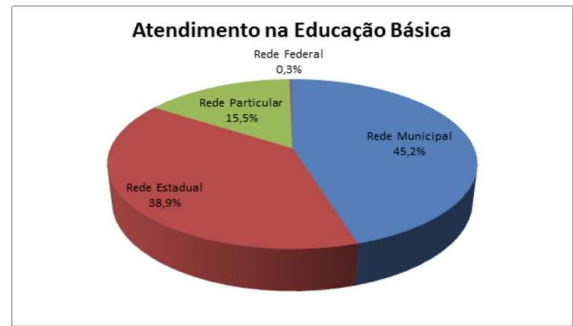
\includegraphics[scale=1.0]{imagens/grafs_1.png}
	\end{center}
	\legend{Fonte: Secretaria Municipal de Educação de Avaré (2014). }

\end{figure}



Texto texto texto texto texto texto texto texto texto texto texto texto texto texto 
texto texto texto texto texto texto texto texto texto texto texto texto texto texto texto 
texto texto texto texto texto texto texto texto texto texto texto texto texto texto texto 
texto texto. 




\begin{figure}[H]
\renewcommand{\figurename}{Gráfico}	
\caption*{ \label{graf2}Gráfico 2 – Distribuição do número de matrículas por etapas da 
educação básica município de Avaré – 2014}
	\begin{center}
	    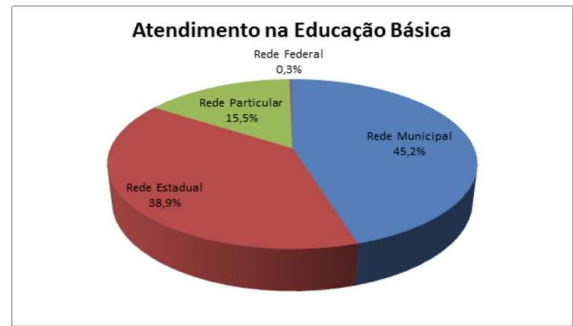
\includegraphics[scale=1.0]{imagens/grafs_1.png}
	\end{center}
	\legend{Fonte: Secretaria Municipal de Educação de Avaré (2014). }

\end{figure}

\renewcommand{\figurename}{Figura}	

\setcounter{secnumdepth}{4}

\titleformat{\paragraph}
{\normalfont\normalsize}{\theparagraph}{1em}\emph{}
\titlespacing*{\paragraph}
{0pt}{3.25ex plus 1ex minus .2ex}{1.5ex plus .2ex}

\paragraph{Título da seção quinária}

Texto texto texto texto texto texto texto texto texto texto texto texto texto texto 
texto texto texto texto texto texto texto texto texto texto texto texto texto texto texto 
texto texto texto texto texto texto texto texto texto texto texto texto texto texto texto 
texto texto texto texto texto texto texto texto texto texto texto texto texto texto texto 
texto texto texto. 

Texto texto texto texto texto texto texto texto texto texto texto texto texto texto 
texto texto texto texto texto texto texto texto texto texto texto texto texto texto texto 
texto texto texto texto texto texto texto texto texto texto texto texto texto texto texto 
texto texto texto texto texto texto texto texto texto texto texto texto texto texto texto 
texto texto texto texto texto texto texto texto texto texto texto texto texto texto texto 
texto texto texto texto texto texto texto texto texto texto texto texto texto texto texto 
texto texto texto texto texto. 

Texto texto texto texto texto texto texto texto texto texto texto texto texto texto 
texto texto texto texto texto texto texto texto texto texto texto texto texto texto texto 
texto texto texto texto texto texto texto texto texto texto texto texto texto texto texto 
texto. 

Texto texto texto texto texto texto texto texto texto texto texto texto texto texto texto texto texto texto texto texto texto texto texto texto texto texto texto texto texto texto texto texto texto texto texto texto texto texto texto texto texto texto texto texto texto texto texto texto texto texto texto texto texto texto texto texto texto texto texto texto texto texto texto texto texto texto texto texto texto texto texto texto texto texto texto texto texto texto texto texto texto texto texto texto texto texto texto texto texto texto texto texto texto texto. 



\begin{figure}[H]
	\caption{\label{fig_arranjo}Arranjo produtivo local da banana orgânica.}
	\begin{center}
	    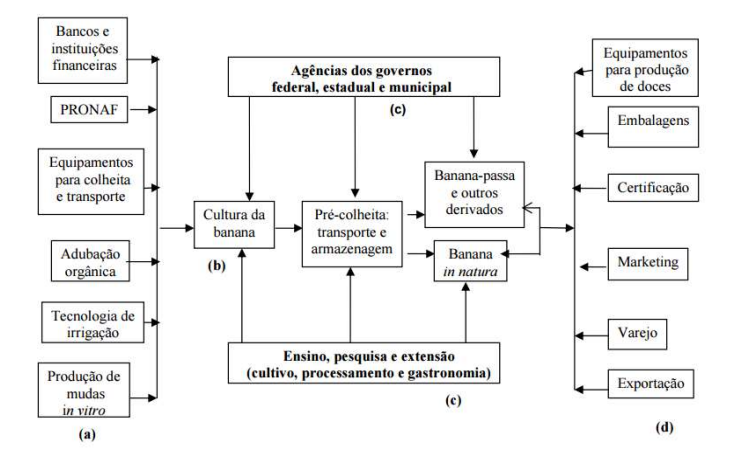
\includegraphics[scale=1.0]{imagens/fig_exemplo.png}
	\end{center}
	\legend{Fonte: \cite{limaarranjo}}
\end{figure}


Texto texto texto texto texto texto texto texto texto texto texto texto texto texto 
texto texto texto texto texto texto texto texto texto texto texto texto texto texto texto 
texto texto texto texto texto texto texto texto texto texto texto texto texto texto texto 
texto. 

Texto texto texto texto texto texto texto texto texto texto texto texto texto texto 
texto texto texto texto texto texto texto texto texto texto texto texto texto texto texto 
texto texto texto texto texto texto texto texto texto texto texto texto texto texto texto 
texto